\section{Romain et le sapin de Noël (3 points)}

%\begin{multicols}{2}
	Romain a un mini sapin de Noël qui décoré de trois guirlandes lumineuses alimentées par une pile. Il mesure les intensités sans le circuit mais son ampèremètre tombe en panne avant qu'il n'ait pu mesurer l'intensité $I_3$ qui traverse la guirlande bleue.
	
	\begin{questions}
		\question Comment peut-il faire pour déterminer $I_3$ sans la mesurer ? 
		\question Quelle valeur trouvera-t-il ?
	\end{questions}

\textbf{Données : } $I_1 = 450 mA$, $I_2 = 450 mA$, $I_4 = 125 mA$

\begin{center}
	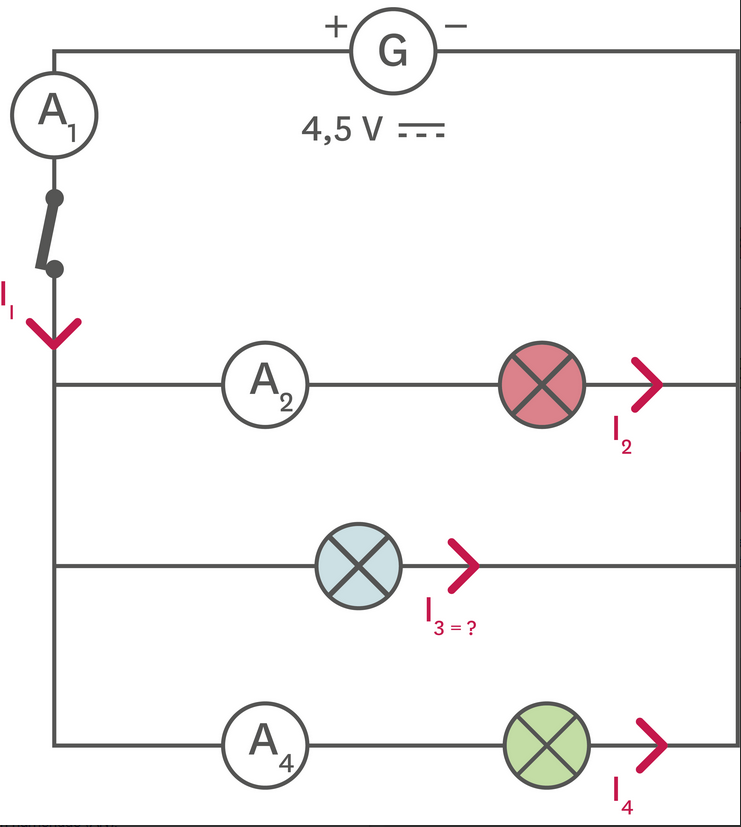
\includegraphics[scale=0.5]{img/sapin}
\end{center}
%\end{multicols}